\chapter{绪论}

\section{研究背景和意义}

自1885年世界上第一辆汽车产生至今,随着科技的进步和人们对于汽车需求量的增加,汽车正在作为重要的交通运输工具,逐步推动着人类各行业的蓬勃发展。根据世界卫生组织发布的《2018年全球道路安全状况报告总结》显示,随着传染病预防和控制的进程的展开,非传染性疾病的死亡人数贡献度在增加,其中道路交通事故是所有年龄段的第八大死亡原因。根据报告调研结果显示,道路交通死亡风险与国家国民收入水平之间存在密切联系,如图1.1所示,中等收入群体国家的道路交通死亡风险率是其他群体国家的四倍多,此外,低收入和高等收入群体国家的道路交通死亡概率,相比较于其国家人口规模和机动车流通数量来说比例出现高畸形。

\begin{figure}[!h]
	\centering
	\includegraphics[height=6.17cm ,width=15.28cm]{figures/图1.1.eps}\\
	\caption{按国家收入类型划分的人口、道路交通死亡人数和登记机动车比例}\label{图1.1}
\end{figure}


导航和媒体设备等车载信息系统(IVISs)现已是汽车的标配产品,用于调节长途驾驶人员的疲劳感和改善乘车人员的体验观感,但是,这些设备的引入将会使得驾驶员分心的诱因增加,从而事故率极大提升。根据2019年NHTSA的报告显示\cite{1},自新型冠状病毒(COVID-19)出现以来,道路上的行车数量减少并没有让交通事故减少,反而有上升趋势,报告指出,交通事故率高居的原因是驾驶员对交通法律法规的漠视和不规范的驾驶行为。

随着汽车持有数量的不断增加,如何提升驾驶者的驾驶环境安全系数,是科学研究人员亟待解决的重要问题。以“驾驶员—车辆—交通环境”三大要素组成的交通系统,驾驶员是交通安全的关键环节。在众多的交通事故中,因驾驶员分心驾驶而导致车祸发生的概率是最高的\cite{2}。

近年来,众多的汽车品牌在自家的汽车产品中不断的增加各种辅助驾驶技术,并在各方面都在提升驾驶员的驾驶安全系数,用于保证乘车人员的生命财产安全,改善交通事故造成的拥堵下现象。高效的行车辅助系统,能够自主学习驾驶人员的行为习惯,对危险的预警反应明显比驾驶者更为迅速,在车辆驾驶人员行为检测方面,比较著名的有百度分心驾驶行为分析系统、滴滴出行的群雁智能出行平台、沃尔沃Ride Pilot辅助驾驶系统等等。

从驾驶者的驾驶行为分析,分心驾驶者的行为在所有影响因素中稳定性是最难得以保证的,同时客观上,在现实的道路交通体系中,驾驶者的主观意识难以有效的进行控制。因此,出于对驾驶人员和乘车人员的安全考虑,迫切的需要外部因素能够对驾驶者的驾驶状态和驾驶行为进行有效的限制约束,使得科研与生活能够相结合,规避交通事故发生一直是科研人员致力于研究的目的所在。

随着传感器精度的不断提升,传感器的体积和重量也在不断的减少,捕获的图像质量急剧提升。得益于深度学习的迅速发展,视觉方面的研究取得了巨大进展,也助力各行各业在迅速发展,其中分心驾驶行为分析研究方面,从任务处理顺序划分为“检测、识别、分类”三步。同时也要考虑自然环境带来的干扰因素,研究在复杂环境下高效的模型识别,及其在车载系统中的跨模态协作等算法的研究,具有更加宽广的理论研究前景和学术研究意义。

在实际使用环境中,以规范驾驶员的驾驶行为为最终目的,分心驾驶行为检测算法的研究在车辆工程发展中一直以来是重中之重。从最开始通过车载方向盘设备内嵌传感器获取电信号开始,科研人员一直在不遗余力地发展分心驾驶行为检测系统,到现在逐渐转变为通过车载摄像头获取图像处理为主,检测驾驶员身体状态信号为辅的跨模态融合的研究中。因其跨模态融合的复杂特性,及其高昂的成本,仅次于其高可靠性的图像处理方式,就图像的学术研究成本和车载设备的成本而言,基于图像的分心驾驶行为检测分析算法研究是很有必要的,能够大大的降低研究的成本,提升产品的推广,更能提高分心驾驶行为检测系统对各种复杂场景的适用性,降低软件研发系统对于硬件设备的依赖性。

从实际应用价值方面,在当今视觉传感器技术如此成熟的环境下,基于图像的分心驾驶行为检测系统能够有效的跨视觉传感器设备,在资源有限的车载设备中稳定高效的运行,而且在保证需求的前提下,向快速进行发展,进而节省车载设备的计算资源,这也是驾驶辅助系统发展的主流之一。

综上所述,基于图像的分心驾驶行为检测算法研究不仅具有很重要的科学研究价值,而且也具有极高的实际应用价值。同时,研究分心驾驶行为检测算法,不仅可以提升驾驶人员的驾驶安全系数的,而且对于减少交通事故的频发具有至关重要的作用,也是市场迅速发展的必然方向。



\section{分心驾驶行为检测技术研究现状}

\subsection{起源}

NHTSA把“任何将驾驶者的驾驶注意力,从车辆驾驶任务中转移的活动”定义为分心驾驶行为,包括使用移动终端接打电话或收发短信、饮食或与车内人员交谈\cite{3}。

NHTSA根据分心源的不同,对车内源分心的造成的交通事故做了深入研究,使用移动终端引发事故的概率是最大的,其次是车载设备,饮食引发的交通事故概率最小\cite{1}。Hossein等人\cite{4}发现在驾驶机动车的过程中,车载娱乐设备和移动终端设备的使用会造成分心驾驶行为,而车载娱乐设备造成的驾驶员操作能力的下降程度远高于移动电话,同时,研究还发现,造成这一结果与驾驶人员的年龄并无关联。Ishida等人\cite{5}通过道路实测数据研究发现,在使用移动终端和接听广播时引起的分心驾驶行为,导致车辆制动距离延长,车辆的平均速度降低,眼球的运动速度缓慢,研究还指出,手持移动设备接打电话或收发短信,明显会影响方向盘的偏转。车外源分心主要包括驾驶过程中被车外广告设计、太阳直射、周围风景等。Redelmeier等人\cite{6}研究发现,车外源分心对驾驶行为安全影响显著,而且相比较于车内源分心而言,车外源分心不可控性更强。

\begin{figure}[!h]
	\centering
	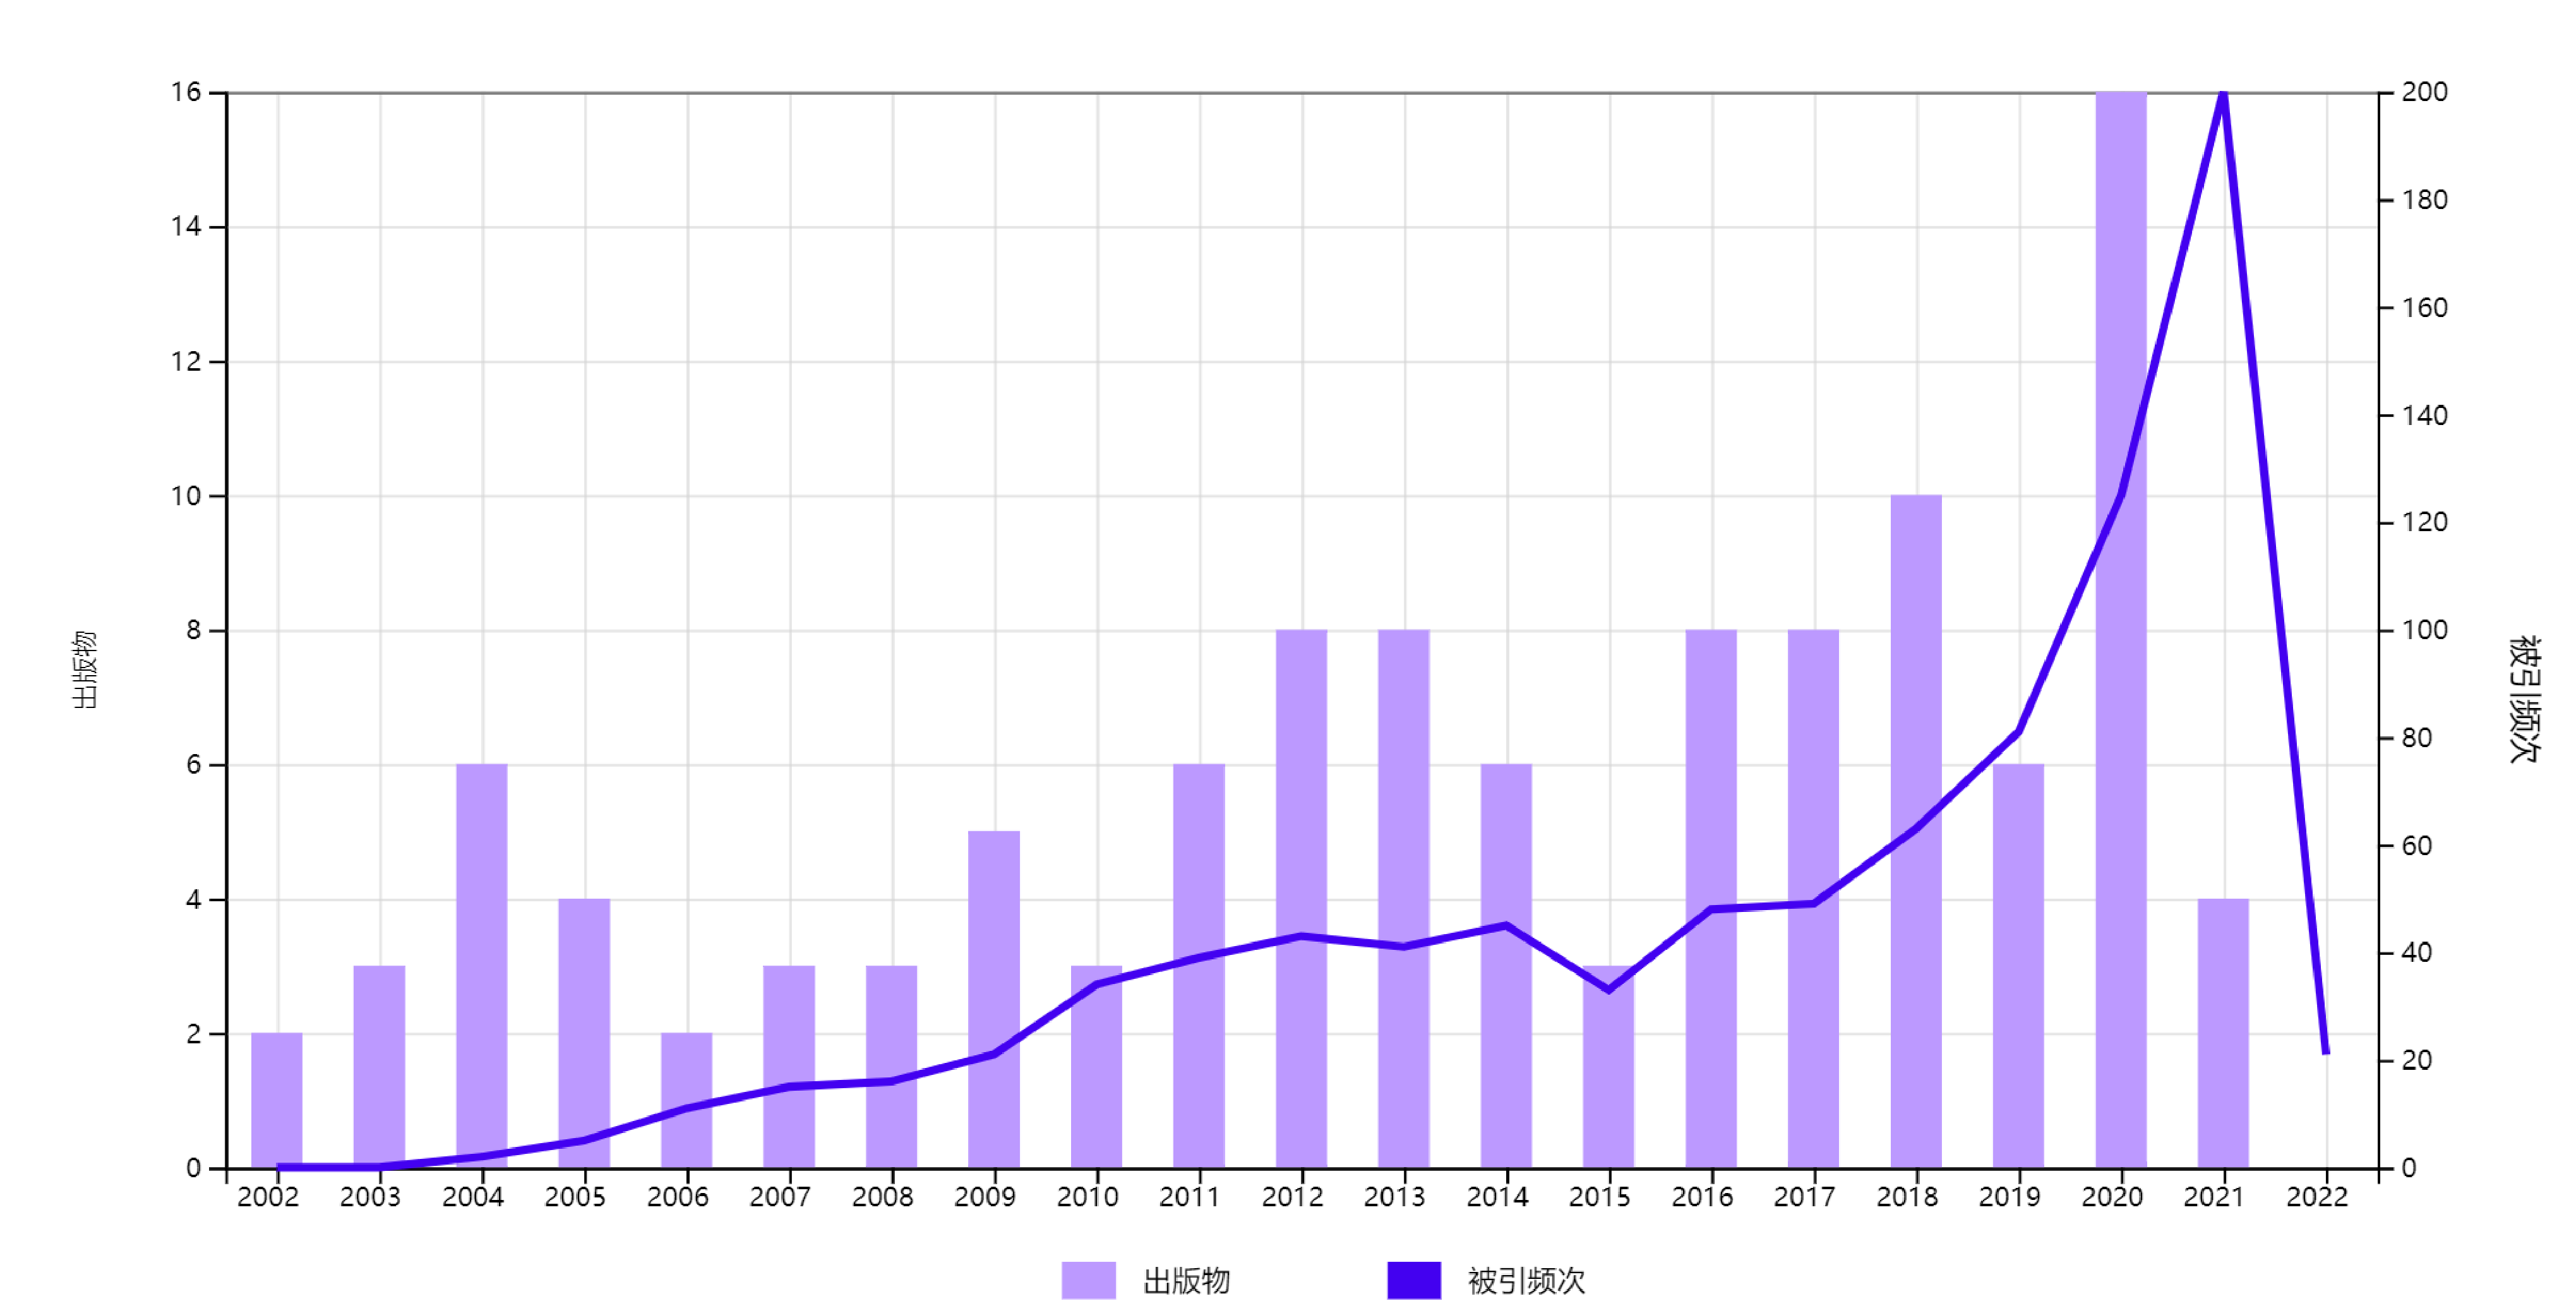
\includegraphics[height=8.24cm ,width=15.5cm]{figures/图1.2.eps}
	\caption{“驾驶行为”研究引文报告}\label{图1.2}
\end{figure}

根据分心驾驶的通道维度区分,听觉分心是由于听觉次任务引起的,视觉分心是指驾驶员由于视觉次任务引起的,例如查看移动设备、导航设备等,当驾驶员视线离开驾驶主任务,也就失去了对车辆状态和道路环境的感知能力,视野离开时间越长危险就越大。Harbluk等人\cite{7}研究车辆驾驶员的驾驶行为时发现,视觉分心时车辆的紧急制动次数明显增加,并且驾驶员对周围环境的敏感度降低,反应时间延长。Ghazizadeh等人\cite{9}研究发现,驾驶员在使用车载设备或移动设备时,会频繁出现视野偏移驾驶主任务超过2s的情况,交通事故率急剧提升。操作分心是指驾驶员在车辆驾驶过程中,手脚资源主动或被动的操作其他设备引起的驾驶员精神不能集中,造成车辆控制能力下降,例如调节中控台、输入导航信息音量等。认知分心是指驾驶员由于认知次任务引起的,驾驶员的注意力机制不在驾驶任务上,大脑潜意识在思考与驾驶任务不相符的事物,例如与乘车人员交谈、接听来电、思考问题等\cite{8}。

多年来,驾驶行为的研究一直是热度很高的方向,包括驾驶行为和驾驶状态,相关研究对于汽车设计制造能够提供理论指导依据,图\ref{图1.2}(来源于:Web of Science引文报告)预示着驾驶行为的研究依旧是理论研究的热门方向,同时也预示着未来汽车的研发创新是理论与实际相结合,相关学者一直致力于此方面的研究。

\subsection{研究现状}

完整的驾驶员分心驾驶行为检测系统主要流程如图\ref{图1.3}所示,由图像采集、图像质量预处理、特征提取、驾驶员驾驶行为分类等四个步骤构成。而且分心驾驶行为检测系统可以与其他辅助驾驶系统相结合,扩宽成一个泛化性更强的综合系统,用以应对复杂多变的外部环境。

\begin{figure}[!ht]
	\centering
	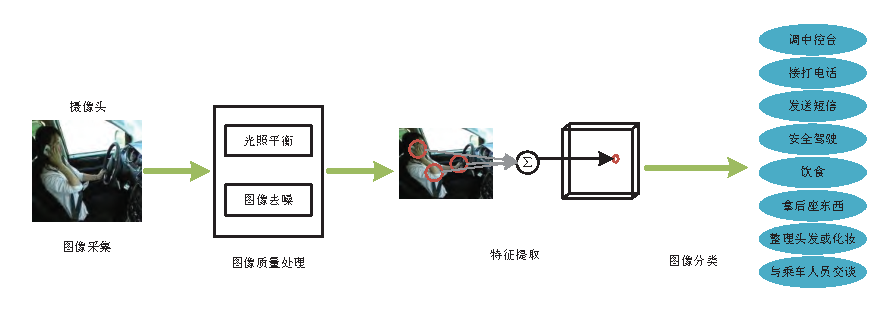
\includegraphics[height=5cm ,width=15.3cm]{figures/图1.3.eps}
	\caption{分心驾驶行为检测算法基本流程}\label{图1.3}
\end{figure}

图像采集装置以光学传感器为主,然而,受限于制造传感器的工艺水准,采集到的数字图像或多或少都会蕴含噪声,对后续任务处理带来了极大的影响,因此图像的噪声检测及去噪是图像处理系统的必备环节。同时,光照也对光学传感器的影响极大,光照的强弱对光学传感器的感知具有很大的干扰特性,干扰过重使得图像将无法检测处理。

数字图像蕴含的所有影响因素都在图像特征提取之前处理,本文统一将其操作归为“图象质量预处理”模块。图像质量预处理过程是以图像获取设备为基础,在图像处理任务之前完成相应的去干扰过程,并非是分心驾驶行为检测特有任务。由于现有光学传感器获取图像的质量得以提升,使得图像噪声的处理不在如以前那么重要,但是在车载等有限资源条件设备上,获取到的图像客观上依旧存在噪声影响,因此在所有的视觉任务中都图像质量预处理环节应该被重视。值得注意的是,现有的论文学术研究中,对于视觉任务的预处理通常是以获得更加出众的目标特征为主要目的,受限于获取数据集图像的数量影响,会进行诸如图像翻转、图像偏转、图像增强等等\cite{10}。这些视觉预处理操作都是在图像质量预处理之后及特征提取之前进行。

驾驶人员的分心驾驶行为检测本质是一个分类任务,遵循分类任务的需求,即提取到容易区分的特征和效果良好的分类器,因此大部分的分心驾驶行为检测的研究都是针对特征提取和分类器展开研究。

根据所处理的图像是连续序列帧还是单一帧,分心驾驶检测的算法研究分为静态、动态两类,而本文所研究是基于模型融合的分心驾驶行为检测算法,故以单帧的静态图像为数据支撑,所以主要是针对静态单帧图像进行分析讨论研究。主流的研究方法可以大致分为以下三类:

\textbf{一、基于统计学方法}

Lansdown等人\cite{11}使用自我评估的调查方式,统计分析了分心驾驶次任务行为,调查显示42\%为阅读短信、41\%为编辑短信和17\%为使用手持移动终端设备通话,这种调查方式,由于操作简单、上手难度较低,在驾驶者行为统计分析邻域得到广泛应用。此方法通常是驾驶员在未驾驶机动车时参与统计,带有一定的滞后性,达不到实际性改善分心驾驶行为检测的目的,即减少分心驾驶行为带来的伤害,避免交通事故的发生。

Jung等人\cite{12}在驾驶员行车过程中,通过ECG传感器提取HRV(心率变化率)信号,计算时域和频域的指标变化,统计评估驾驶员疲劳状况。Almahasneh等人\cite{28}构建了驾驶员认知分心检测模型,使用奇异值分解(SVD)提取特征,支持向量机(SVM)分类,超越了其他模型。

奔驰公司的驾驶员注意力辅助系统(Attention Assist)融合了多种复杂的车辆制动信息及周围道路信息,使用统计分类的方式,综合分析驾驶员注意力和疲劳度,用于提升驾驶员的健康驾驶效率\cite{7}。关伟等人\cite{14}通过研究驾驶者的行为信息,统计分析出脑电信号(EGG)与各种分心驾驶行为之间的数学关系。

\textbf{二、机器学习方法}

(1)	分心驾驶行为特征提取

分心驾驶行为的特征提取是分心驾驶行为分析归类的重要环节,提取到的特征越全面,分心驾驶行为检测系统的性能越好,然而受限于实际提取特征算法的性能和运算设备的计算能力,并非所有特征都会被提取,因此研究方法主要是在尽可能提取高效特征,改进分类算法的设计。总的来说,有效的分心驾驶行为特征应该具有以下几个共同特点:

\begin{itemize}
	\item 完整的行为特征能够表征该类的本质特点。
	\item 具有较强的鲁棒性,能够有效地去除光照、噪声、遮挡的等等以及与分心驾驶行为无关的冗余信息。
	\item 特征的表征数据表示形式紧凑,避免出现过高维度数据。
	\item 不同类型的表征数据特征具有良好的区分度。
\end{itemize}

传统的机器学习方法在提取驾驶行为特征时主要有以下三类方式:

%基于表征特征的方法是以像素为基础,将变换系数映射为驾驶行为的特征,其中,这些像素将会反映驾驶员底层的信息,体现了驾驶人员的细节信息。传统经典的方法有:非矩阵分解(Nonnegative Matrix Factorization,NMF)\cite{24}、Gabor小波变化法\cite{18,19}、局部纹理模式(Local Texture Features,LTP)\cite{17}、多尺度几何分析算法(Multiscale Geometric Analysis,MGA)\cite{21}、局部二值模式(Local Binary Patterns,LBP)\cite{15,16}、方向梯度直方图(Histogram of Oriented Gradients,HoG)\cite{20}、尺度不变算法(Scale Invariant Feature Transform,SIFT)\cite{22}、子空间分析方法\cite{23}和卷积核方法(Convolution Kernel,CK)等等。

基于表征特征的方法是以像素为基础,将变换系数映射为驾驶行为的特征,其中,这些像素将会反映驾驶员底层的信息,体现了驾驶人员的细节信息。传统经典的方法有:非矩阵分解\cite{24}、Gabor小波变化法\cite{18,19}、局部纹理模式\cite{17}、多尺度几何分析算法\cite{21}、局部二值模式\cite{15,16}、方向梯度直方图\cite{20}、尺度不变算法\cite{22}、子空间分析方法\cite{23}和卷积核方法等等。


基于几何特征的方法以驾驶员的几何姿态模型为基础,通过检测姿态和运动轨迹来表征驾驶员的行为信息。2011年,张等人\cite{25}使用安装在仪表盘上的摄像头,捕获驾驶员的驾驶行为图像,从图中提取面部、嘴巴和手部特征,并应用隐藏条件随机场(HCRF)模型来检测手机的使用情况。2014年,Berri等人\cite{26}应用支持向量机(SVM)模型来检测手部和面部位置,并通过驾驶员的正面图像来检测手机的使用情况。2015年,Craye等人\cite{27}通过分析Kinect传感器捕获的RGB-D图像数据,利用AdaBoost和隐式马尔可夫链模型对驾驶员分心驾驶行为进行分类。

基于混合特征的方法是由前两者方法相结合而成,即几何方法建立驾驶员身体姿态的模型,表征方法则是注重于疲劳度的微观姿态变化情况。薛雷等人\cite{29}通过模拟驾驶实验,结合脑电波信号的变化与驾驶员驾驶主观感受的评价指标,建立了驾驶员疲劳的分类模型,受限于特征人为提取的方式,对熟练度具有很高的要求。

(2)	分心驾驶行为分类

驾驶人员的行为分类是整个系统的最后环节,也是最为重要的环节。驾驶人员分心检测的目标是判断待检测图像的特征与训练数据集中的某一类分心类别特征之间的相似程度,选取相似度最高的一类作为结果输出相应类别。常见机器学习特征分类算法有以下几类:

K近邻分类算法(K-Nearest Neigbors,K-NN),其中K是可调的参数,评价算法分类性能的好坏关键在于计算机能否寻找到适合的K指。K-NN分类器从测试数据集中寻找K个最邻近样本数据,把已经训练好的标签作为K个最近样本标签。

支持向量机(Support Vector Machine,SVM)是基于VC维理论,在样本中间使用支持平面进行划分样本类别的算法,样本类别被分为两类。

AdaBoost首先,通过反复训练找出权重分布最佳的弱分类器,其次,使用弱分类器调整相应参数,最后,将多个弱分类器将整合为一个强分类器。

人工神经网络,可以通过训练样本进行反复训练,自我学习最佳到模型状态,以求能够在规则中寻求到最佳的隐性条件。由于其优越的特性,在诸多问题中使用也越来越广泛。


\textbf{三、深度学习方法}

基于传统机器学习的驾驶员分心驾驶检测算法通常是利用特定的规则将提取的特征进行分类,此类方法对于分心驾驶行为检测的复杂多变环境的实用性能力较差,例如检测驾驶人员的变动,不同的身体比例,使得传统机器学习的算法实用性降低。然而,基于机器学习在驾驶员理想姿态图像上取得了优异的成绩,在自然环境下的驾驶员分心检测表现欠佳,很难满足当今时代对于现有问题的处理时效、处理性能和鲁棒性等等多方面要求。近些年以深度学习为主的的驾驶员分心驾驶行为检测研究,以其优异的性能和对外界噪声的强抗干扰能力,并逐渐在车载系统中开发应用。在驾驶员分心驾驶行为检测领域,经常使用的深度学习网络结构有如下几种:

(1)	卷积神经网络

卷积神经网络(Convolutional Neural Network,CNN),是分心驾驶检测任务中目前应用最广泛的一种网络结构,将局部特征通过共享权重有效的进行关联,加快模型的训练速度。近些年,许多高效网络模型相继被提出,而且也在分心驾驶检测领域取得了优异的成绩,诸如VGGNet、ResNet、ViT等等。近年来分心驾驶行为研究逐渐倾向于行为个体,因此借助于神经网络在计算机视觉方向的发展,夏瀚笙等人\cite{30}通过采集人体关键点,使用VGG16和ResNet50卷积神经网络,进行分心驾驶行为的检测研究。Baheti等人\cite{31}采用卷积神经网络VGG16,通过修改VGG网络,将模型准确度提升到95.54\%。

(2)	循环神经网络

%循环神经网络(Recurrent Neural Network,RNN)是时序性的网络模型,以处理连续图像特征为主,需求时间上的特征关系。Streiffer等人\cite{32}提出了不同模型的混合模型DarNet,将卷积神经网络(CNN)、支持向量机(SVM)、循环神经网路(RNN)进行融合,用于研究驾驶员的分心状态。

循环神经网络(Recurrent Neural Network,RNN)是时序性的网络模型,以处理连续图像特征为主,需求时间上的特征关系。Streiffer等人\cite{32}提出了不同模型的混合模型DarNet,将卷积神经网络、支持向量机、循环神经网路进行融合,用于研究驾驶员的分心状态。



综上所述,分心驾驶行为的研究还是以机器学习方法为主,其中提取的特征是分类准确与否的前提条件,然而,特征提取工作依赖于个人经验,研究工作仍存在巨大的挑战,相关算法也受制于相关设备及其具体环境的影响,其鲁棒性也不能够得到有效保证。近些年,随着深度学习算法应用在计算机视觉方向的研究,使得研究分心驾驶行为检测趋向于低成本,高可靠性驱动,适配于版本老旧的设备成为了可能。深度学习依靠其端到端的学习训练方式,深受广大研发人员的热衷,出现了诸多的新颖方式,诸如,集成学习方式,采用多种网络结构的模型,提取多种不同特征,用以提升分类任务的性能,但由于集成学习的方式训练难度较高,很难应用于具体的工程实践中,因此提出了采用基于注意力机制的网络模型来提升分类任务的性能,其本质上仍是集成学习的方式。

\subsection{分心驾驶行为数据集}

早期的关于驾驶的研究是通过测量身体机能电信号,进而对获取的信号进行处理分析,通过统计学手段,筛选出特定要求的阈值信号,作为检测依据,因此并没有能够留下珍贵的数据集资源,使得未来的后续研究难以复现当时的具体实验数据,对于学术研究难以推广到具体生产环境中。
	
\begin{figure}[!h]
	\centering
	\includegraphics[height=9.58cm ,width=14.73cm]{figures/图1.4.eps}\\
	\caption{StateFarm分心行为机器类别样本标签分布}\label{图1.4}
\end{figure}

2002年,吕宝粮教授等人创办了仿脑计算与智能研究中心(BCMI),推出了SEED、SEED-IV和SEED-VIG三个数据集,其中SEED-VIG是关于疲劳度驾驶数据集,数据集是以EGG脑电信为主,根据统计人体在不同条件下的脑电波动情况,选出合理的阈值,用于研究疲劳驾驶时人体脑电波的信号变换情况。

2014年03月,Shabnam等人\cite{35},在文章中提出了YAWDD数据集,对于驾驶人员困意检测的研究,提供了便利研究,数据集的下载研究是开源的。数据集是通过车载图像捕获设备来收集驾驶人员的打哈欠图像,是一段30fpsAVI样式的视频,包含了640×480,24bit的RGB图像。

2016年03月,Kaggle机构推出了StateFarm数据集\cite{36},数据集是从车载图像捕获设备上获取的,收集自26名司机日常驾驶图像。图\ref{图1.4}展示了数据集中每个类别数据量的分布情况,训练集22424张图像和测试集79726张图像两部分组成,训练集已经使用label-class进行了分类,包含了10个分心类别,然而,测试集并没有进行任何分类。StateFarm的特点是测试集的图像数量远多于训练集图像数量,想对而言对训练的模型会产生极大的影响。

2018年06月,国立清华大学(NTHU)计算机视觉实验室收集的驾驶员嗜睡视频数据集,包括训练、验证和测试三部分,共还有36个不同种族的数据提供人员,在昼夜照明条件下,提供各种模拟场景的姿态图像,整个数据集总时长约5430分钟。

2018年12月,在2018NIPS智能交通系统机器学习研讨会上,Abouelnaga等人\cite{37}在会议上,提出现实场景下的分心驾驶行为研究方法,并提供了AUCD2分心驾驶行为检测数据集,并开源与诸位科研人员共同使用。与StateFarm数据集类似,AUCD2数据集拥有10个分心类别。数据是在同一辆车辆上,使用图像捕获设备进行采集,拥有12978张训练图像和4332张测试图像,测试机拥有标签并按照类别进行了分类规整。

2019年03月,百度推出了自家的驾驶行为分析AI智能检测系统,基于驾驶室捕获的驾驶员行为图像,通过终端设备上传至百度云AI计算平台,分析图像并回传结果数据,进行解析。采用的是客户端与云计算相结合的方式,客观上存在延时,并且由于百度推出的服务是商业行为,因此非常遗憾的是并没有任何的数据资料公开用于算法学习和研究。

2020年04月,奥迪公布了综合数据集A2D2(Audi Autonomous Driving Dataset)\cite{34},供科研人员下载研究。该数据集主要来自德国街道,记录的数据是以时间为基准,包括3D点云数据和RGB图像。

综上所述,使用深度学习进行视觉研究,需要庞大的数据,对于分心驾驶行为方面的研究,可开源使用的数据集更是少之又少,大多数公司高额的数据使用费用使得分心驾驶行为研究者望而却步。虽然在奥迪公司2020年公开自己采集的数据集开始,拥有的3D点云标记数据,由往常的2D静态图像的研究开始转变为动态的3D图像数据研究。然而,A2D2数据集的2.3TB庞大数据量存储本身就是一个很困扰的问题,且计算机的GPU计算能力现今而言,很难饱和的达到A2D2数据集的计算量,难以发挥数据集的特性。综合考虑实际情况,选择AUCD2数据集和StateFarm数据集作为本文的研究数据集。

\section{本文主要研究内容及论文结构}

在2016年,kaggle举办了第一个基于分心驾驶行为检测数据集StateFarm的竞赛,也是目前唯一个分心驾驶行为检测研究的竞赛,随后论文也接踵而至,使得分心驾驶行为的研究由原先从生理电信号,开始逐步借助深度学习的便利演变为基于视觉的研究,这也是目前诸行业的研发趋势。所以,本文的总体目标是研究基于静态图像的分心驾驶行为检测算法研究。

\subsection{研究内容}

一个完整的分心驾驶行为检测系统包括图像采集、噪声检测、去噪处理、分心驾驶行为特征提取以及行为分类等诸多部分组成(如图\ref{图1.5}所示)。本文旨在研究分心驾驶行为检测的主体算法部分,考虑到工程模拟中图像存在的噪声,因此加入了噪声检测和去噪处理部分。本文的研究重点是模型融合提取特征和高区分度的孤立中心损失函数部分两部分,针对以上两个关键点展开了细致研究,并分析问题的所在,提出相应的解决策略,具体研究内容包含以下几部分:

(1)	问题分析

针对分心驾驶行为检测具体问题,依据现今阶段的发展情况,摒弃传统的统计学信号处理方法,在机器学习的特征分类方法和深度学习的特征分类方法的选择中,因以下优点,即基于视觉庞大数据量,以及深度学习的模型自收敛方式和端到端训练方式的优点等因素,综合考虑下,最终选择使用深度学习方式来解决相应问题。

(2)	数据集预处理

对已有的数据进行预处理,主要目的是为了模拟不同的场景、不同的图像采集设备和不同时间段获取到图像存在的质量差异性问题。针对不同的图像质量差异性问题,寻找影响模型准确度的噪声因素,统计分析影响阈值,以实际统计效率为主,选择图像噪声的预处理方式。

(3)	模型融合

如何高效的提取数据特征,一直以来是一个重点关注问题,在此问题上,出现了诸多方式,但都存在先天性的缺陷,机器学习手工特征提取很依赖操作人员的经验,单一的深度学习模型存在的特征提取不全面问题。因此,采用多个模型进行特征的提取,对所提取特征进行综合判别,提升分心驾驶行为检测算法的性能,提高模型应对复杂多变环境的抗干扰性能。

(4)	损失函数改进

高区分度的类别分类器在训练时尤为重要,模型特征最终能否将采集的图像特征进行准确的区分,分类器是重中之重。然而,训练模型的分类数据集通常存在一个不可避免的问题,即数据集类别数量不平衡带来的类别多样本特征对类别少样本在角度域挤压问题,针对此问题,展开研究,通过改进损失函数来克服,进一步提升模型整体的鲁棒性。

\begin{figure}[!h]
	\centering
	\includegraphics[height=7.27cm ,width=12.21cm]{figures/图1.5.eps}\\
	\caption{分心驾驶行为检测流程与论文章节结构}\label{图1.5}
\end{figure}

\subsection{论文章节安排}

本文主要章节与分心驾驶行为检测算法的对应关系如图\ref{图1.5}所示,具体章节内容安排如下:

第一章:阐述分心驾驶行为检测研究的背景和意义,介绍了分心驾驶行为的技术发展历程,分析了国内外分心驾驶行为检测研究的发展现状、研究必要性和应用价值,并介绍了国内外分心驾驶研究的数据集情况及其发展历程,最后介绍了本文研究框架及其主要研究内容。

第二章:一个完整的系统将设计多个环节,会使用到诸多技术,本文在图像预处理环节将会采用现有的技术,所以本章会简单的介绍涉及到的相关经典算法和基础理论,包括图像噪声检测估计方法、图像去噪技术。

第三章:首先介绍了单个网络模型,分析讨论单个网络模型的特点,及其对应存在的问题,仔细分析对比不同网络模型对驾驶分类的影响,进一步设计综合优化的模型。详细进行了实验对比,验证模型融合方法与最新的诸多分心驾驶模型之间的性能差异,实验结果表明模型融合方法确实能够提升分心驾驶行为检测算法的性能,并且具有很好的鲁棒性。

第四章:首先介绍了卷积神经网络特征区判别的原理,同时分析了各种提升神经网络特征判别的技术优点和不足之处,进一步提出本文改进Softmax分类器的必要性。然后从中心损失函数出发,分析分类器的原理和不足之处。遵循“类间特征分离,类内特征聚集”的指导思想,设计了孤立中心损失函数方法,通过大量的实验进行验证损失函数的有效性。

第五章:结合论文第二章、第三章和第四章内容,设计一个完整的分心驾驶行为检测系统的工程模拟方案,根据测试数据,反馈相应的信息,完成整个分心驾驶行为检测算法的模拟工作。

第六章:对本文所进行的主要研讨内容和相关工作做了总结。同时,针对现有分心驾驶行为检测算法研究存在的技术性难点问题,和可深入内容点,进行未来研究发展方向的展望。






